% Created by Chris Chronopoulos (chrono@leaflabs.com) on 20140930
% 

% ***********************************************************
% ******************* PHYSICS HEADER ************************
% ***********************************************************
% from http://www.dfcd.net/articles/latex/latex.html
% ***********************************************************
% Version 2
\documentclass[11pt]{article} 
\usepackage{amsmath} % AMS Math Package
\usepackage{amsthm} % Theorem Formatting
\usepackage{amssymb}	% Math symbols such as \mathbb
\usepackage{graphicx} % Allows for eps images
\usepackage{multicol} % Allows for multiple columns
\usepackage[dvips,letterpaper,margin=0.75in,bottom=0.75in]{geometry}
\usepackage{amsmath}
\usepackage{graphics}
\usepackage{graphicx}
\usepackage{epsfig}
\usepackage{verbatim}
\usepackage{listings}
\usepackage{enumerate}
\usepackage[authoryear]{natbib} % can't get this to work?
\usepackage{hyperref} % i think there's a conflicting command here?
 % Sets margins and page size
% \pagestyle{empty} % Removes page numbers
\makeatletter % Need for anything that contains an @ command 
\renewcommand{\maketitle} % Redefine maketitle to conserve space
{ \begingroup \vskip 10pt \begin{center} \large {\bf \@title}
	\vskip 10pt \large \@author \@date \end{center}
  \vskip 10pt \endgroup \setcounter{footnote}{0} }
\makeatother % End of region containing @ commands
%\renewcommand{\labelenumi}{(\alph{enumi})} % Use letters for enumerate
% \DeclareMathOperator{\Sample}{Sample}
\let\vaccent=\v % rename builtin command \v{} to \vaccent{}
\renewcommand{\v}[1]{\ensuremath{\mathbf{#1}}} % for vectors
\newcommand{\gv}[1]{\ensuremath{\mbox{\boldmath$ #1 $}}} 
% for vectors of Greek letters
\newcommand{\uv}[1]{\ensuremath{\mathbf{\hat{#1}}}} % for unit vector
\newcommand{\abs}[1]{\left| #1 \right|} % for absolute value
\newcommand{\avg}[1]{\left< #1 \right>} % for average
\let\underdot=\d % rename builtin command \d{} to \underdot{}
\renewcommand{\d}[2]{\frac{d #1}{d #2}} % for derivatives
\newcommand{\dd}[2]{\frac{d^2 #1}{d #2^2}} % for double derivatives
\newcommand{\pd}[2]{\frac{\partial #1}{\partial #2}} 
% for partial derivatives
\newcommand{\pdd}[2]{\frac{\partial^2 #1}{\partial #2^2}} 
% for double partial derivatives
\newcommand{\pdc}[3]{\left( \frac{\partial #1}{\partial #2}
 \right)_{#3}} % for thermodynamic partial derivatives
\newcommand{\ket}[1]{\left| #1 \right>} % for Dirac bras
\newcommand{\bra}[1]{\left< #1 \right|} % for Dirac kets
\newcommand{\braket}[2]{\left< #1 \vphantom{#2} \right|
 \left. #2 \vphantom{#1} \right>} % for Dirac brackets
\newcommand{\matrixel}[3]{\left< #1 \vphantom{#2#3} \right|
 #2 \left| #3 \vphantom{#1#2} \right>} % for Dirac matrix elements
\newcommand{\grad}[1]{\gv{\nabla} #1} % for gradient
\let\divsymb=\div % rename builtin command \div to \divsymb
\renewcommand{\div}[1]{\gv{\nabla} \cdot #1} % for divergence
\newcommand{\curl}[1]{\gv{\nabla} \times #1} % for curl
\let\baraccent=\= % rename builtin command \= to \baraccent
\renewcommand{\=}[1]{\stackrel{#1}{=}} % for putting numbers above =
\newtheorem{prop}{Proposition}
\newtheorem{thm}{Theorem}[section]
\newtheorem{lem}[thm]{Lemma}
\theoremstyle{definition}
\newtheorem{dfn}{Definition}
\theoremstyle{remark}
\newtheorem*{rmk}{Remark}
% added by CKC
\newcommand{\amom}{\mathcal{L}}
\newcommand{\flux}{\mathcal{F}}
\newcommand{\laplacian}[1]{\nabla^2 #1}


% ***********************************************************
% ********************** ENDcit HEADER *************************
% ***********************************************************

\usepackage{bm}

\title{Willow GUI User Guide}
\date{\today}

\begin{document}
\maketitle

%%%%%%%%%%%%%%%%%%%%%%%%%%%%%%%%%%%%%%%%%%%%%%%%%%%%%%%%%%%%%%%%%%%%%%%%%%%%%%%%%

\section{Introduction}
\label{sec_intro}

This is the user guide for the Willow GUI --- a desktop application for interacting with Willow, a 1024-channel electrophysiology system developed by LeafLabs (www.leaflabs.com) in collaboration with MIT's Synthetic Neurobiology Group (SNG). This document, which is contained in the source code repository in \texttt{docs/user\_guide/}, contains information for end-users. Developers should check out the developer's guide, which can be found in \texttt{docs/dev\_guide/}.

%%%%%%%%%%%%%%%%%%%%%%%%%%%%%%%%%%%%%%%%%%%%%%%%%

\section{System Overview}
\label{sec_overview}

Willow is based on a Spartan 6 FPGA which collects and routes data from up to 32 amplifier/digitizer chips (Intan RHD2132), each chip sampling 32 channels of electrophysiology signals. The primary purpose of the hardware is to record all 1024 channels of data directly to an SSD, which is connected via SATA interface to the Willow board. A photograph of the bare hardware, connected and ready to record from a single headstage, is shown in Figure~\ref{fig_hw}.

\begin{figure}[h!]
\begin{center}
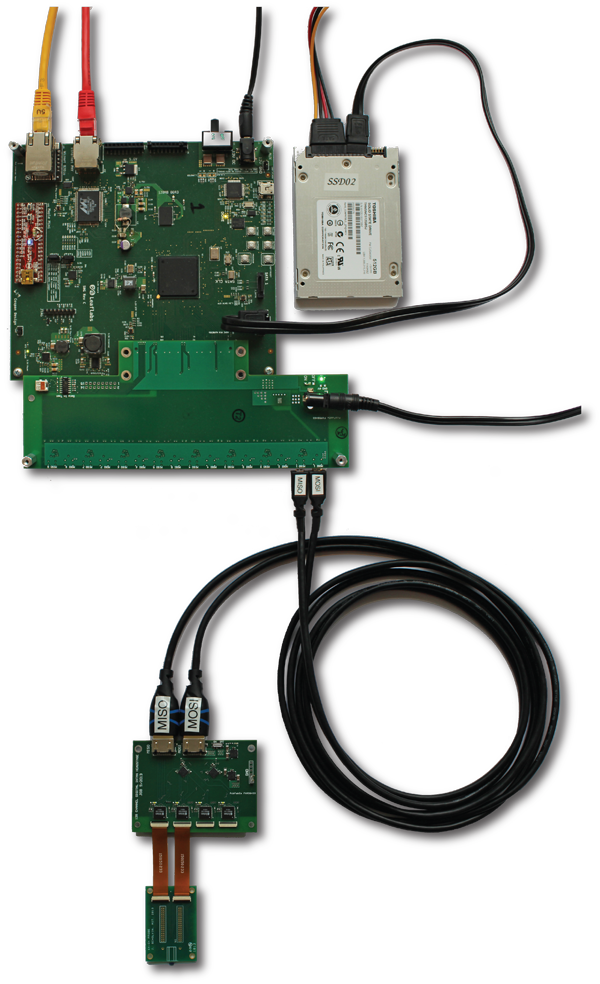
\includegraphics[width=6cm]{screenshots/full_setup.png}
\end{center}
\caption{Willow hardware with a single headstage connected.}
\label{fig_hw}
\end{figure}

The Willow board communicates over TCP and UDP connections with a workstation computer running a daemon server called \texttt{leafysd}. All interactions with the hardware go through the daemon, which exposes an interface based on Google's Protocol Buffers (protobuf). The daemon repository includes command-line utilities for sending and receiving protobuf messages to and from the daemon. The GUI was designed to replace the command-line workflow with a more accessible and streamlined graphical approach.

There are many layers to the full Willow system; to learn more about them in detail, see \texttt{wired-leaf-docs/user\_guide}. For the end-user, however, it is sufficient to be familiar with the basic architecture of the system. Namely, that the only robust mode of data acquisition is recording, which saves data directly to the SSD, and not to the workstation. To tighten the feedback look for data validation, there are other modes of acquisition (namely streaming and snapshots) which route data directly to the workstation, but these are not robust to data loss. For scientific experiments, the workflow is: record to SATA disk, then transfer over to a workstation for analysis. This is further explained in Section~\ref{sec_usage}.

%%%%%%%%%%%%%%%%%%%%%%%%%%%%%%%%%%%%%%%%%%%%%%%%%%%%%%%%%%%%%%%%%%%%%%%%%%%%%%%%%

\section{Setup}
\label{sec_setup}

This setup guide assumes you have already installed the daemon and configured your network; if not, refer to the Willow user guide in \texttt{wired-leaf-docs/user\_guide}.

\subsection{Obtaining the GUI}
\label{sec_setup_obtaining}

To access the GUI repository, you'll need to be given permissions on the server --- to request access, email \texttt{neuro@leaflabs.com}. Once you have permissions, you can clone the repo like so

\vspace{5mm}
\texttt{\$ git clone git@git.leaflabs.com:sng-gui}
\vspace{5mm}

\subsection{Dependencies}
\label{sec_setup_deps}

Before running the GUI, install these mandatory dependencies:

\vspace{5mm}
\texttt{\$ sudo apt-get install python-numpy python-matplotlib python-qt4 python-h5py \textbackslash}

\hspace*{20mm}\texttt{python-progressbar}
\vspace{5mm}

\subsection{Configuration}
\label{sec_setup_config}

The GUI uses a configuration file, \texttt{src/parameters.py}, which stores variables related to the daemon installation, data storage, and other parameters. Before running the GUI, open \texttt{src/parameters.py} in an editor and modify the \texttt{DAEMON\_DIR} and \texttt{DATA\_DIR} variables to point to the locations of the \texttt{sng-daemon} repo and the preferred top-level data directory on your system.

%%%%%%%%%%%%%%%%%%%%%%%%%%%%%%%%%%%%%%%%%%%%%%%%%

\section{Usage}
\label{sec_usage}

To run the GUI:

\vspace{5mm}
\texttt{\$ cd src/}

\texttt{\$ ./main.py}
\vspace{5mm}

\noindent
The GUI will present its main window (Figure~\ref{fig_mainwindow}), which consists of the status bar, the button panel, and the message log. The daemon is automatically started in the background, with \texttt{stderr} and \texttt{stdout} redirected to \texttt{log/eFile} and \texttt{log/oFile}, respectively. The message log should display a line indicating that the daemon was started successfully.

\begin{figure}[h!]
\begin{center}
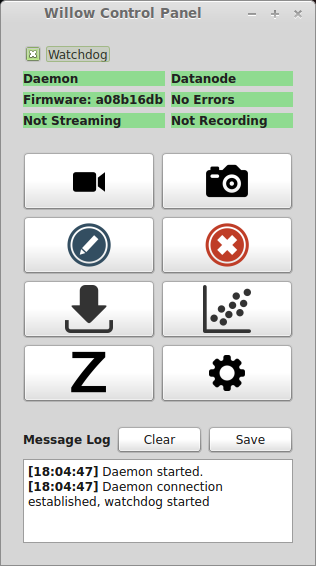
\includegraphics[width=6cm]{screenshots/mainwindow.png}
\end{center}
\caption{GUI main window, immediately after startup, showing the status bar at the top, the button panel in the middle, and the message log at the bottom.}
\label{fig_mainwindow}
\end{figure}


%%%%%%%%%%%%%%%%%%%%%%%%

\subsection{Status Bar}
\label{sec_usage_statusbar}

The status bar is an array of labels at the top of the main window, which indicates the status of the daemon and the hardware. The status bar is updated by a watchdog process which pings the datanode once every second, and evaluates the response to determine daemon status, datanode status, firmware version, error conditions, streaming state, and recording state. The general color code for the labels is: green for ``good/normal state'', orange for ``bad state, something is wrong'', and gray for ``unknown state''. For example, if the datanode is unresponsive, its label will turn orange and the labels below it will turn gray to indicate an unknown state. Similarly, if the daemon is unresponsive, its label will turn orange and all labels below it will turn gray. These conditions are shown in Figure~\ref{fig_statusbar}.

\begin{figure}[h!]
\begin{center}
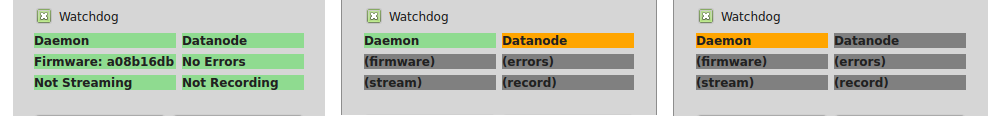
\includegraphics[width=17cm]{screenshots/statusbar_threestates.png}
\end{center}
\caption{Status bar in three states: Daemon up and connected to Datanode, showing firmware version, error state, and streaming/recording states (\textit{left}); Daemon up but datanode unresponsive (\textit{center}); Daemon down or unreachable, hardware state unknown (\textit{right}).}
\label{fig_statusbar}
\end{figure}

The firmware label, when green, will show the firmware version as a 32-bit hexadecimal number. The error label beside it indicates whether an error condition is present on the datanode. If so, this label will turn orange and display the value of the top-level error register, which is a bitmask of the error states of the sub-modules on the FPGA. If an error condition comes up on the datanode, you'll need to reboot it to clear the errors. Hardware-related bug reports can be sent to \texttt{info@leaflabs.com}, and should include both the firmware version and the error state bitmask as context.

The ``Stream'' label indicates the streaming state of the datanode: green for idle, and blue for streaming. Similarly, the ``Record'' label beside it is green for idle, but turns red while recording and additionally indicates the current disk usage as a percentage in real time. These states --- streaming and recording --- are determined from the hardware registers on the datanode, and are therefore robust to daemon and/or GUI crashes.

The Watchdog process can be disabled by un-checking the ``Watchdog'' box at the top of the status bar. This should rarely be necessary, but may free up some bandwidth during streaming or transfer operations on slow workstations. The status bar will no longer be updated while the Watchdog is disabled.

%%%%%%%%%%%%%%%%%%%%%%%%

\subsection{Message Log}
\label{sec_usage_messagelog}

\begin{figure}[h!]
\begin{center}
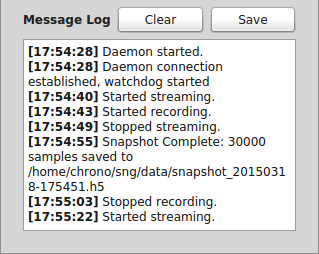
\includegraphics[width=8cm]{screenshots/msgLog.png}
\end{center}
\caption{The message log, showing a list of actions taken, with timestamps.}
\label{fig_statusbar}
\end{figure}

At the bottom of the main window is the message log, which displays and logs messages from the GUI. Examples of messages include success/failure reports from requested actions, status updates from background threads, and general errors. Each message is prepended with a timestamp of the form \texttt{HH:mm:ss}. The message log can be cleared, or saved to a log file using the buttons at the top-right. Message logs are saved to the \texttt{log/} subdirectory by default, but can be saved anywhere by navigating the presented file dialog.

The message log is intended to serve as a supplement to the experimentalist's lab notebook, logging the actions taken --- and their results --- to help contextualize the data for future analysis.

%%%%%%%%%%%%%%%%%%%%%%%%

\subsection{Button Panel}
\label{sec_usage_buttonpanel}

At the center of the main GUI window is the button panel, containing 8 buttons with symbolic icons. These buttons are your starting point for all the capabilities offered by the GUI. Mousing over a button will display a tooltip which describes its action.

\subsubsection{Streaming}
\label{sec_usage_buttonpanel_streaming}

Streaming is the real-time visualization of data from the Intan chips. When streaming, the data acquired from the ADC's is routed directly to the GUI, without being saved to SATA. Currently, users can view one channel at a time, as a scrolling waveform in a stream window.

To launch a stream window, click the ``Launch Stream Window'' button in the Button Panel. You will be presented with a dialog to configure the stream parameters. Fill in the channel number you wish to view, the plotting range, and the refresh rate --- or, accept the default values and click ``OK''. The stream window will appear (Figure~\ref{fig_streamwindow}) in an idle state. To start/stop the stream, use the ``Start'' and ``Stop'' buttons. You can also navigate the plot, even while streaming, using the Navigation Toolbar at the bottom of the stream window. To undo/redo navigation changes, use the back and forward arrows; to return to the original view, click the home icon.

Live streaming in matplotlib is reasonably CPU intensive, so you may want to pause the stream while running other tasks within the application. Adjusting the ``refresh rate'' parameter in the stream dialog may help alleviate performance issues.

\begin{figure}[h!]
\begin{center}
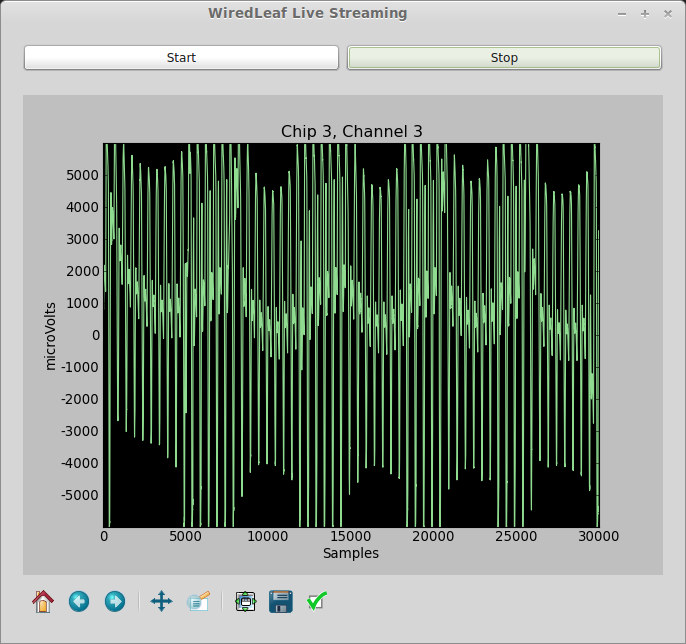
\includegraphics[width=14cm]{screenshots/streamwindow.png}
\end{center}
\caption{Stream window showing 60 Hz noise from a bare Intan chip.}
\label{fig_streamwindow}
\end{figure}

\subsubsection{Snapshots}
\label{sec_usage_buttonpanel_snapshot}

A snapshot is a short (\textless~10 second) acquisition of board samples (all 1024 channels) which is saved directly to the workstation. It is essentially a stream which gets saved to a file (HDF5 format by default) to be analyzed offline. Like streaming, taking a snapshot does not involve the SATA drive, so you can take snapshots without worrying about overwriting your experiment on disk.

To take a snapshot, first make sure that any Stream Windows are stopped; then click the ``Take Snapshot'' button in the Button Panel. You will be presented with a dialog to configure the snapshot. Fill in the number of seconds you wish to acquire, and the filename you want to save to, and click ``OK''. The default filename is generated from the ``Data Directory'' parameter in your settings (see Section~\ref{sec_usage_buttonpanel_settings}) and a timestamp taken at the moment you clicked ``Take Snapshot'' --- the format is \texttt{dataDir/snapshot\_YYYYMMDD-hhmmss.h5}, so the filename should be unique up to 1 second of granularity.

The snapshot dialog also gives you the option to ``Plot when finished'' by checking the box in the lower-left corner. If this is selected, then after the snapshot is saved, the GUI will automatically import the file and present it in a Plot Window (refer to Section~\ref{sec_usage_plot} for information on using the Plot Window).

\subsubsection{Recording}
\label{sec_usage_buttonpanel_recording}

Recording is the acquisition of data directly to the SATA disk. It is the only acquisition mode that is guaranteed to be robust, and is intended for scientific experiments. To start a recording, click the ``Start Recording'' button in the Button Panel. The corresponding label in the status bar will turn from green to red, and the label will begin displaying the disk usage. Accurate reporting of disk usage is depending on the ``Datanode Storage Capacity'' parameter in your settings (see Section~\ref{sec_usage_buttonpanel_settings}). To stop recording, click the ``Stop Recording'' button.

\vspace{5mm}
\noindent \textbf{IMPORTANT:} Every time you click ``Start'', the system will start recording from the beginning of the disk, over-writing any previous experiments you may have recorded. In this sense, the disk acts as a temporary (non-volatile) buffer for experimental data. If you've just recorded an experiment and want to preserve the data, it is recommended that you \underline{transfer} the data over to your workstation immediately after stopping recording (see Section~\ref{sec_usage_buttonpanel_transfer}). If storage space is an issue on your workstation, an alternative is to remove the SATA disk and label it, thus repurposing the disk buffer as an archival system.

\subsubsection{Transferring Experiments}
\label{sec_usage_buttonpanel_transfer}

The transfer function is used to transfer an experiment from the SATA disk to the workstation's file system. An experiment must be transferred before it can be analyzed --- but even if analysis is not immediately necessary, it is wise to transfer important experiments over as soon as they are recorded, because (as explained in Section~\ref{sec_usage_buttonpanel_recording}) experiments on disk are in danger of being over-written by subsequent recordings.

To perform a transfer, click the ``Transfer Experiment'' button in the button panel. You will be presented with a dialog to specify how much of the experiment you wish to transfer (either the entire experiment, or a subset), and the target filename. Click ``OK'' to begin the transfer. An infinite progress bar will appear until the transfer is complete --- once it is, a success message will appear in the message box.

A couple of things to consider before initiating a transfer: First, transferred experiment files can be quite large (as large as the datanode storage capacity, i.e. 1~TB), so make sure you have the space on your workstation to store these files. Second, transfer times are approximately equal to recording times; if your recording lasted $n$ minutes, you can expect to wait $\sim n$ minutes for a transfer to complete. In order to avoid daemon contention, you will be locked out of any GUI interactions until the transfer is complete.

\begin{figure}[h!]
\begin{center}
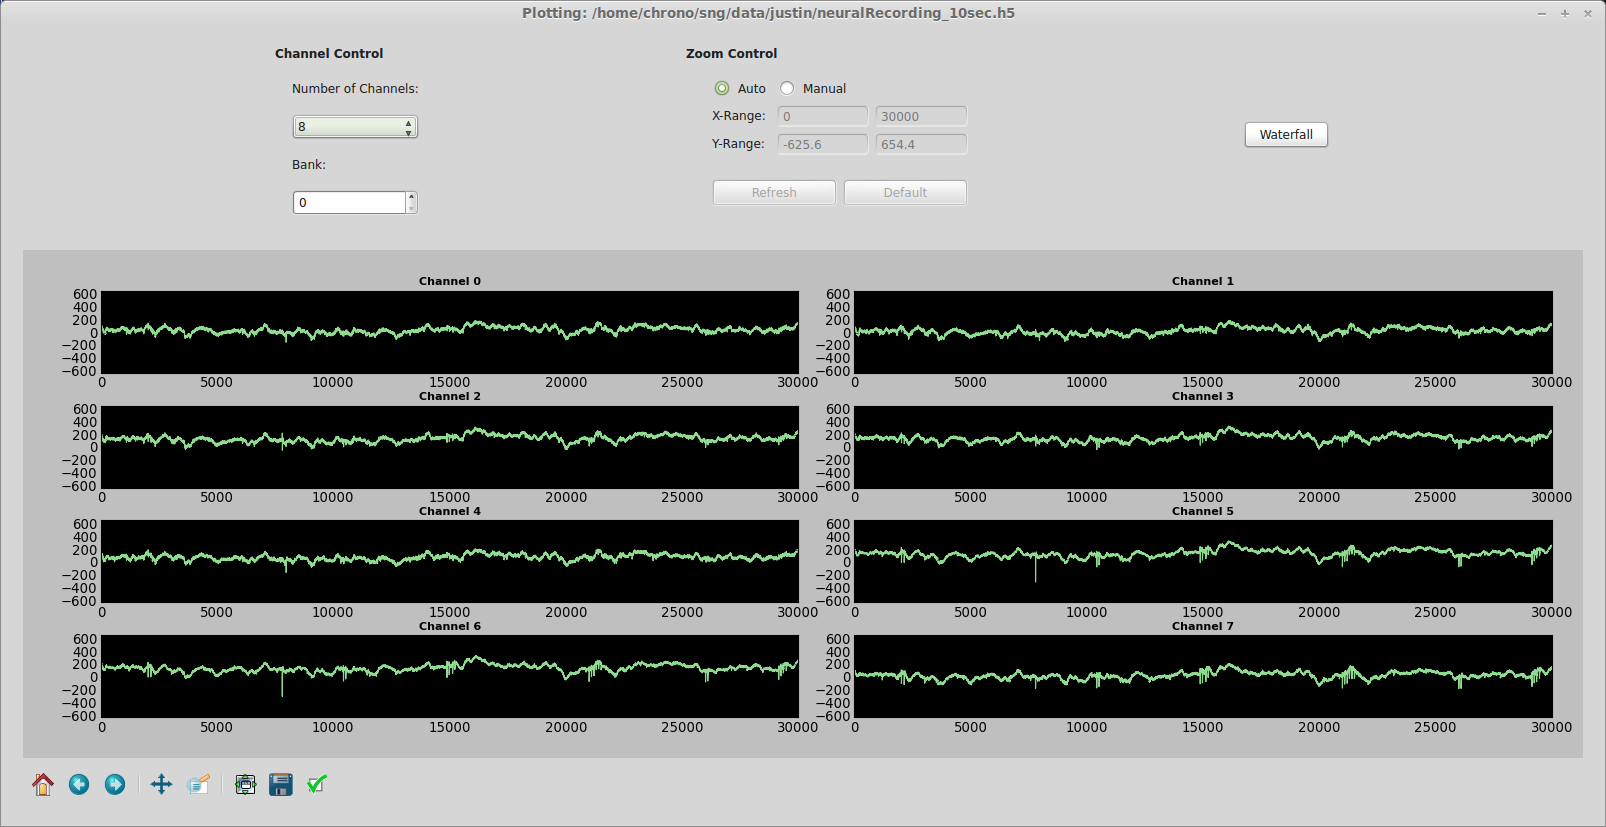
\includegraphics[width=17cm]{screenshots/plotwindow.png}
\end{center}
\caption{The Plot Window.}
\label{fig_plotwindow}
\end{figure}

\begin{figure}[h!]
\begin{center}
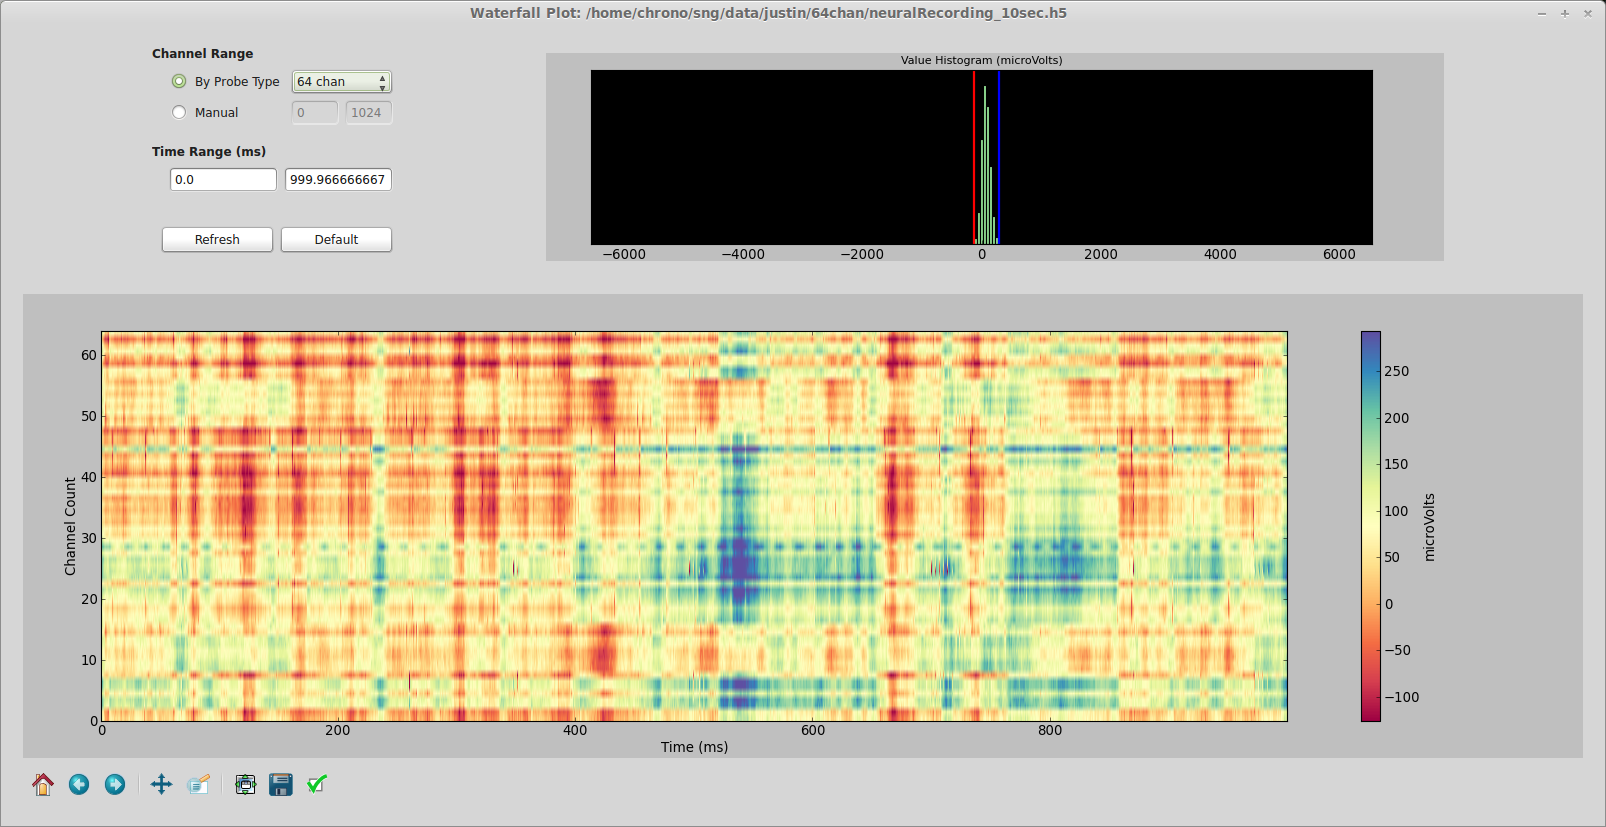
\includegraphics[width=17cm]{screenshots/waterfall.png}
\end{center}
\caption{Waterfall Plot Window.}
\label{fig_waterfall}
\end{figure}

\begin{figure}[h!]
\begin{center}
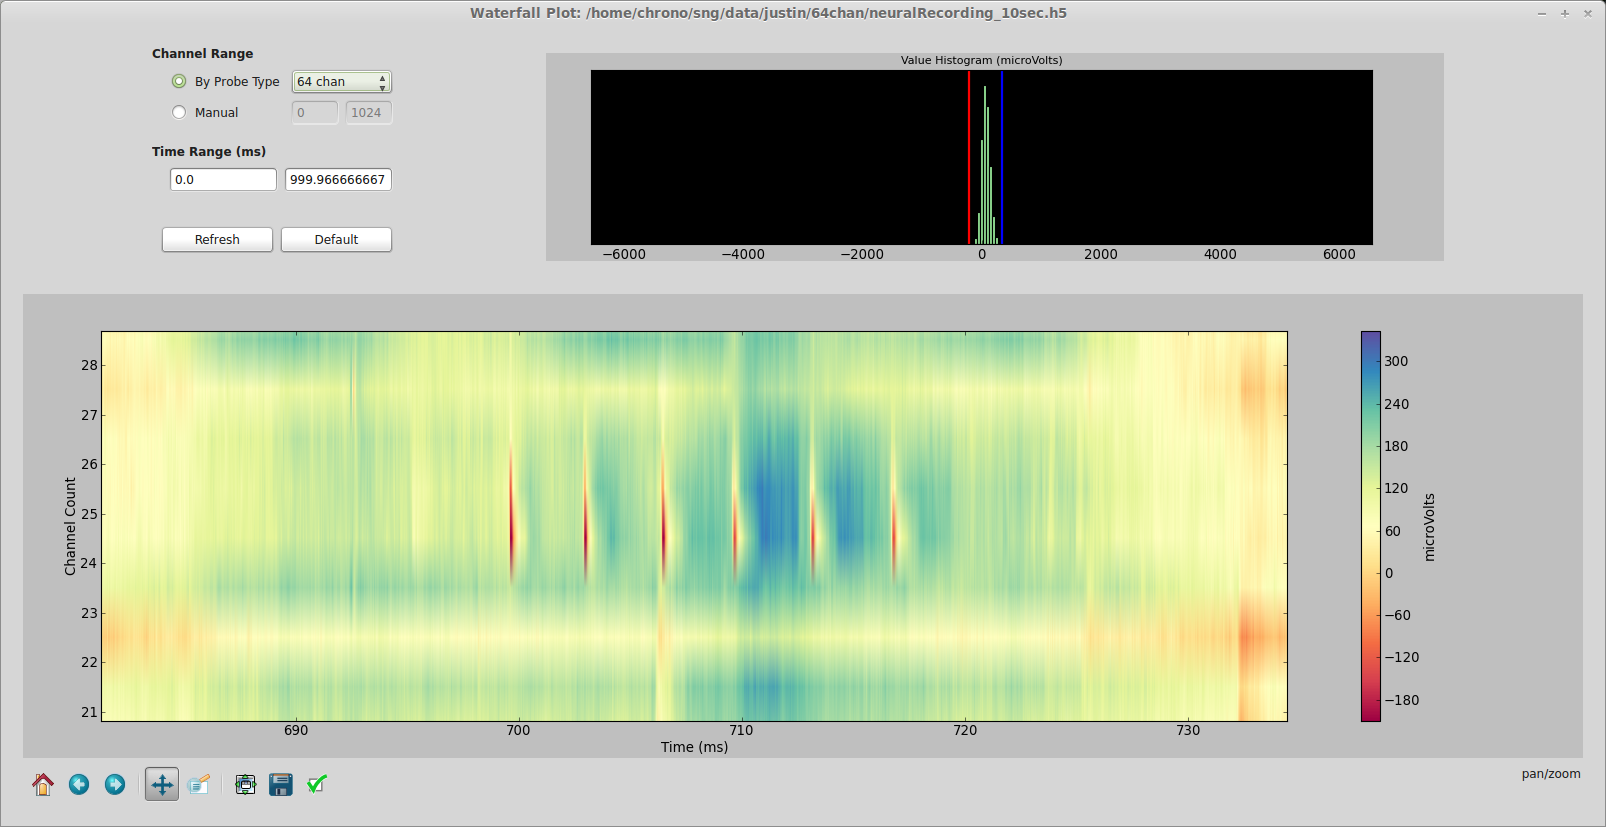
\includegraphics[width=17cm]{screenshots/waterfall_zoom.png}
\end{center}
\caption{A train of 6 spikes, shown on several channels in the Waterfall Plot.}
\label{fig_waterfall_zoom}
\end{figure}
\subsubsection{Plotting Data}
\label{sec_usage_buttonpanel_plot}

In addition to its primary purpose as the driver software for the Willow hardware, the GUI also offers some basic plotting utilities for exploring datasets. To plot a dataset (either a snapshot or a recording), click the ``Launch Plot Window'' button in the button panel. In the file dialog that appears, select the file you wish to import, and click ``OK''. Then enter how much data to import: either the entire file, or a subset. Be aware of the time and memory requirements before initiating an import --- 1 second of data can take nearly 10 seconds to import, and large datasets can quickly consume memory resources. To prevent excessive memory consumption, the GUI will refuse to import datasets larger than the ``Dataset Import Limit'' parameter in the settings (see Section~\ref{sec_usage_buttonpanel_settings}.

The dataset will be imported in a background thread, with a progress dialog indicating the status of the operation. Once complete, a Plot Window will appear (Figure~\ref{fig_plotwindow}), showing the data as an array of 1-dimensional waveforms. A control panel at the top allows you to adjust how many channels are shown at once, which bank of channels is currently being displayed, and the range of the plotting axes. A ``bank'' here represents a contiguous, ordered set of $n$ channels, where $n$ can range from 1 to 16. To page through banks, use the spinbox in the control panel --- when activated, it can be controlled using the arrow keys on your keyboard.

The ``Zoom Control'' section allows you to set the plotting range of \textbf{all} plots in the window simultaneously. By default, the zoom mode is ``Auto'', which looks at the current bank of channels and chooses a $y$-range based on its min and max; the auto-range updates every time you advance banks, or change the number of channels displayed. In ``Manual'' mode, you can set exactly the $x$-range and $y$-range of all the plots in the array --- just enter the extrema and click ``Refresh''. Another way to adjust the plots is by using the Navigation Toolbar at the bottom of the window. This allows you to zoom in on one plot in particular, leaving the others unchanged. To get back to the zoom settings defined by the ``Zoom Control'' group, just click the home icon.

Near the top-right corner of the Plot Window, you'll find a button labeled ``Waterfall''. Click here to launch the Waterfall Plot Window. The Waterfall Plot Window (Figure~\ref{fig_waterfall}) shows \textbf{all} the data from a given import, in a 2-dimensional color plot. The $x$-axis is time (with units in sample number), the $y$-axis is channel number, and color represents signal (voltage), with values indicated by the colorbar on the right. When you first open the Waterfall Plot Window, it will show the entire 1024-channel dataset. If any of the channels were not connected to a live Intan chip, they will show up as zeros, which will appear as a large red band on the Waterfall Plot. To zoom in on the channels of interest, adjust the ``Channel Range'' parameters in the control panel at the top --- this can be done manually, or automatically by probe type. To zoom in on a window of time, adjust the ``Time Range'' parameters. As usual, you can also zoom into subregions of the plot by using the Navigation Toolbar at the bottom. Finally, to adjust the limits of the color mapping, an interactive value histogram is provided at the top-right of the Waterfall Plot Window. The red and blue vertical lines represent the lower and upper limits of the color map, and these can be adjusted by left-clicking and right-clicking, respectively, on the histogram. In Figure~\ref{fig_waterfall_zoom}, we have used these techniques to zoom in on a spike train that registered across several channels.


\subsubsection{Impedance Testing}
\label{sec_usage_buttonpanel_impedance}

The Intan headstages offer impedance testing functionality which can be accessed from the GUI. Click the ``Run Impedance Test'' button on the button panel --- this will present a dialog where you can choose to measure the impedance of a single channel, or of all channels in sequence. If you choose ``Single Channel'', the process will take about 10 seconds, and the result will be posted on the message log. If you choose ``All Channels'', the loop will run for about 3 minutes, and the result will be saved in a time-stamped \texttt{.npy} file, also reported in the message log. In ``All Channels'' mode, you also have the option to ``Plot When Finished'', which will bring up a plot window showing the impedance results across all channels (see Figure~\ref{fig_impedance}). All impedance measurements are taken at $f = 1\text{ kHz}$.

\begin{figure}[h!]
\begin{center}
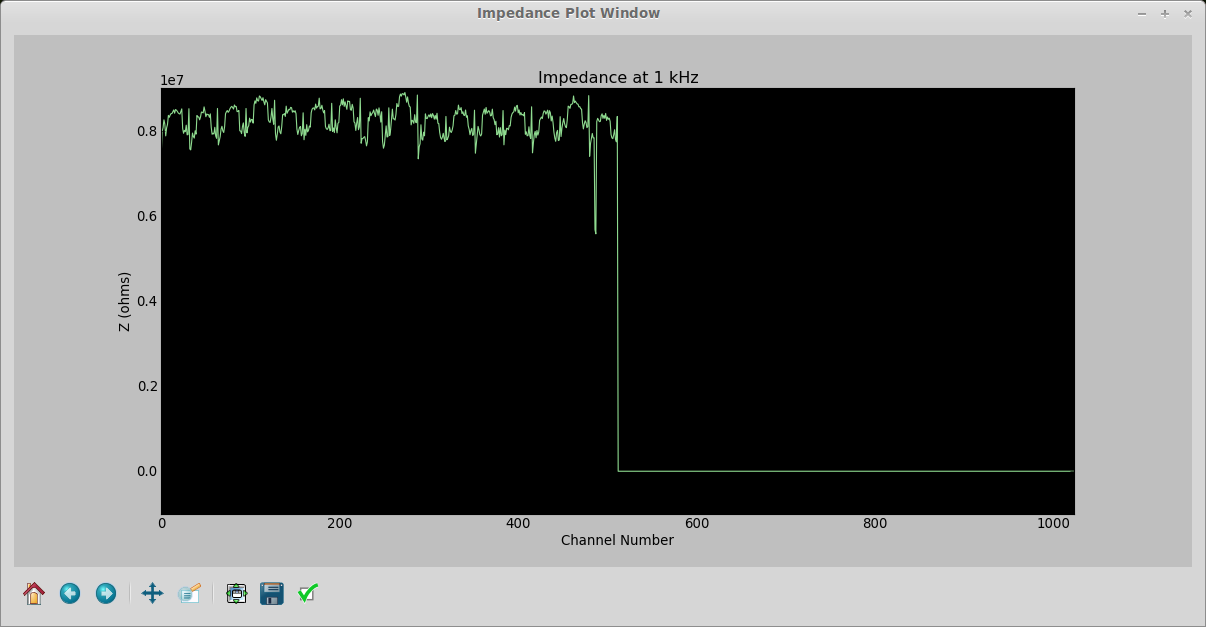
\includegraphics[width=15cm]{screenshots/impedance.png}
\end{center}
\caption{Impedance results from a measurement taken with 4 of 8 headstages bare headstages connected. As expected, channels 0-511 show an approximate, 32-channel periodicity from the PCB traces, and channels 512-1023 are dead.}
\label{fig_impedance}
\end{figure}

\subsubsection{Settings}
\label{sec_usage_buttonpanel_settings}

Blah blah settings.


%%%%%%%%%%%%%%%%%%%%%%%%%%%%%%%%%%%%%%%%%%%%%%%%%

\end{document}





